\documentclass[10pt,twocolumn,letterpaper]{article}

\usepackage{cvpr}
\usepackage{times}
\usepackage{epsfig}
\usepackage{graphicx}
\usepackage{lipsum}
\usepackage{amsmath}
\usepackage{amssymb}
\usepackage{multirow}
\usepackage{epstopdf}
\usepackage{xcolor}
\usepackage[breaklinks=true,colorlinks=true,bookmarks=false,pagebackref]{hyperref}
\usepackage{balance}
\usepackage{longtable}
\usepackage{booktabs}
\usepackage{array}
\usepackage{breqn}
\newcolumntype{R}{>{\raggedleft\arraybackslash}p{3.5mm}}
\newcolumntype{E}{>{\raggedleft\arraybackslash}p{5.3mm}}
\usepackage{array}

\newcommand\blfootnote[1]{%
  \begingroup
  \renewcommand\thefootnote{}\footnote{#1}%
  \addtocounter{footnote}{-1}%
  \endgroup
}

\usepackage{caption}
\usepackage{subcaption}

\DeclareMathOperator*{\argmin}{\arg\!\min}

\usepackage[breaklinks=true,bookmarks=false]{hyperref}

\cvprfinalcopy % *** Uncomment this line for the final submission

\def\cvprPaperID{****} % *** Enter the CVPR Paper ID here
\def\httilde{\mbox{\tt\raisebox{-.5ex}{\symbol{126}}}}

% Pages are numbered in submission mode, and unnumbered in camera-ready
%\ifcvprfinal\pagestyle{empty}\fi
\setcounter{page}{1}
\begin{document}

%%%%%%%%% TITLE
\title{Object Detection with R-CNN}

\author{Albert Haque \qquad Fahim Dalvi\\
Computer Science Department, Stanford University \\
{\tt\small \{ahaque,fdalvi\}@cs.stanford.edu}
}

\maketitle
%\thispagestyle{empty}

%%%%%%%%% ABSTRACT
\begin{abstract}
\vspace{-2mm}
We evaluate the performance of the R-CNN algorithm with extensive hyperparameter tuning and several feature representations. Using a multivariate bounding box regression, we achieve 60.0\%, 22.4\%, and 22.6\% AP for the cat, car, and person classes, respectively. This resulted in a mAP of 35.0\%. To accelerate feature extraction, we use a multi-machine multi-GPU cluster. Additionally, we extend R-CNN to extract foregorund silhouettes from a video using GrabCut image segmentation.
   \vspace{-2mm}
\end{abstract}


%%%%%%%%% BODY TEXT
\section{Introduction \& Related Work}
% TODO: Make sentences flow better (i.e. don't always say In [3] the authors do X Y Z. Use more transitions and state negatives of each method and suggestion solution with another paper, etc.)
Exhaustive search \cite{dalal2005histograms, harzallah2009combining, viola2004robust} and segmentation based approaches \cite{carreira2010constrained, endres2010category}, have both been used for object detection in the past. While exhaustive search attempts to search for all object proposals in an image, segmentation attempts to construct object proposals from the underlying pixels. More recently, the resurgence of convolutional networks has prompted research to fuse object detection with deep learning.

Exhaustive search is computationally expensive and thus requires constraints to prune the search space and reduce the number of considered locations, at the cost of completeness. In \cite{felzenszwalb2010object}, Felzenszwalb \etal performed an exhaustive search using HOG features and a linear SVM. This resulted in excellent object detection performance. To better guide the exhaustive search, in \cite{lampert2009efficient}, Lampert \etal used an appearance model, combined with a branch and bound technique, to remove scale, aspect ratio, and grid constraints from the previous exhaustive search formulation. However, their method still requires evaluation on over 100,000 proposals \cite{alexe2010object}.

Segmentation-based approaches generate a foreground/background segmentation and predict objects based on their foreground segmentations. In \cite{gu2009recognition}, the authors segment objects based on a parts model. Each part is described by appearance and shape features. In \cite{arbelaez2011contour}, Arbelaez \etal use a contour detector which has been shown to provide excellent results. Although segmentation methods perform well, they are often computationally expensive.

% Deep learning for detection related work

Ever since Krizhevsky \etal demonstrated the success of convolutional networks \cite{krizhevsky2012imagenet}, the computer vision community has flocked to deep learning solutions for various classification, tracking, and detection tasks \cite{sermanet2013overfeat, ouyang2014deepid, iandola2014densenet, erhan2014scalable}. 

In \cite{szegedy2013deep}, Szegedy \etal modify the AlexNet architecture to solve a regression task, namely bounding box regression. Inspired by this, Girshick \etal use convolutional network features to train a pipeline consisting of a classifier and regression step, called R-CNN \cite{girshick2014rich}.  Szegedy \etal revisit the R-CNN and reduce the computational overhead in \cite{szegedy2014scalable}. Additionally, several other studies have reduced the computational cost for region proposals while maintaining, if not improving, detection performance (e.g. Fast R-CNN \cite{girshick2015fast} and \cite{szegedy2014scalable}).

In \cite{hariharan2014simultaneous}, Hariharan \etal use a R-CNN for simultaneous detection and segmentation. In \cite{zhang2014part}, the authors fuse a parts based model with convolutional networks for fine-grained category detection. 

\section{R-CNN Algorithm}

%Selective search, CNN extraction, SVM training, hard mining, bounding box regression, etc.

In \cite{girshick2014rich}, Girshick \etal investigate object detection by decomposing the task into three components: (i) region proposal generation, (ii) feature extraction, and (iii) detection.

\textbf{Region Proposal Generation}. Region proposals can be generated by a variety of methods (\eg objectness \cite{alexe2012measuring}, multiscale combinatorial grouping \cite{arbelaez2014multiscale}, category-independent object proposals \cite{endres2010category}, constrained parametric min-cuts \cite{carreira2012cpmc}, and edge boxes \cite{zitnick2014edge}). Girshick \etal propose to use selective search -- a hierarchical grouping method used to generate region proposals \cite{uijlings2013selective}. Selective search uses a greedy algorithm to iteratively group similar regions together. On average, this results in 2,300 region proposals per image.

\textbf{Feature Extraction}. A convolutional network (\eg AlexNet \cite{krizhevsky2012imagenet} or VGG-Net \cite{simonyan2014very}) is used to extract features from each region. Because the CNN requires a fixed size input, Girshick \etal warp each region proposal and break aspect ratio. Regions are resized to $227 \times 227$ pixels such that there are exactly $p=16$ pixels (in the new $227 \times 227$ warped region) around the original region. After performing a forward pass, the activations at the fully-activated layers (typically fc6 or fc7) are used as features. These features are then used during training and test-time detection. A comparison of features and network architectures is in Section \ref{sec:experiments}.

\textbf{Detection}. Given the features for each image, during test time, detection is performed in three steps. First, each region proposal is classified using a class-specific SVM trained by hard-negative mining. Second, a class-specific regression is performed to predict a new bounding box. Third, non-maximal suppression is run to combine bounding boxes with high intersection-over-union (IoU) overlap.

\section{Technical Approach}\label{sec:technical_approach}

\subsection{Features}

We compare two convolutional network architectures, namely the JonNet and VGG-16 \cite{simonyan2014very} network. For JonNet, we use the fc6\_ft rectified activations -- resulting in 512 features per region. For the VGG-16 network, we use both the fc6 and fc7 rectified activations -- resulting in 4096 features per region. Our rationale for selecting the VGG-16 network is based on the empirical finding that a network with better CNN classification performance is correlated with better detection performance when used as a feature extractor \cite{girshick2015fast}.

\subsection{Object Classifiers}

We implemented and evaluated the performance of several object classifier designs. We tested various strategies for hard mining (e.g. keeping $N$ most difficult negatives from training, both as a constant and percentage proportional to the number of positive examples). We further experiment by removing a proportion of easy negative examples. This led to many more hard negatives (as we did not have a hard limit on the number of negatives that remain after removing easy examples), but no significant gain in performance was observed.

%We implemented and analyzed several design choices for our object classifiers. We tested various strategies for hard mining like keeping $N$ hardest negatives seen so far for training, where $N$ was either a constant or proportional to the number of positive examples. We also tested just removing a certain proportion of the easy negatives. This led to a lot more hard negatives (as we did not have a hard limit of how many negatives remain after removing the easy ones), but no significant gain in performance.

We experiment with several training strategies such as re-training after a constant number of images have been seen or after we have collected some preset number of hard negatives. Several pre-processing schemes were implemented such as feature standardization and zero-mean unit-variance normalization. We also experimented with $\ell_1$ and $\ell_2$ SVM regularization.

%We also adopted various retraining strategies, like retraining after a constant number of images and retraining after we have collected some preset number of hard negatives since the last training. We tested various pre-processing schemes like standardization and zero-mean unit-variance normalization. We also used different regularization schemes like $\ell_1$ and $\ell_2$ regularization.%

\subsection{Bounding Box Regression}

We implement four ridge regressors for each class as outlined in \cite{girshick2014rich}. Since the underlying data distribution for each of the regressors is comparable, we use the same regularization penalty for each regressor. For training examples, we use all bounding boxes that have an overlap of at least $0.6$ with any ground truth bounding box in the current image.

\begin{figure*}
	\vspace{-5mm}
        \centering
        \begin{subfigure}[b]{0.24\textwidth}
                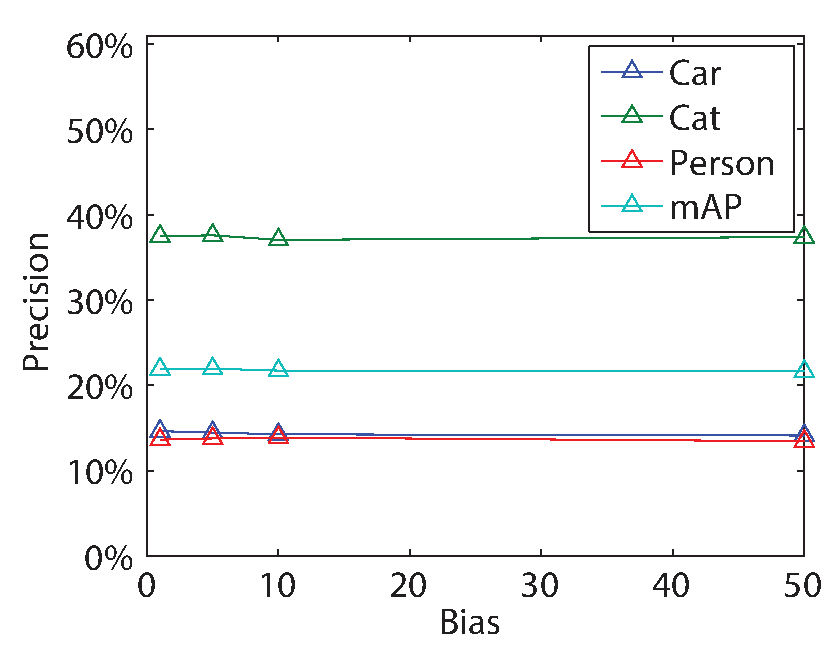
\includegraphics[width=\textwidth]{figures/tuning/bias.eps}
                \caption{SVM Bias}
                \label{fig:bias}
        \end{subfigure}%
        ~ 
        \begin{subfigure}[b]{0.24\textwidth}
                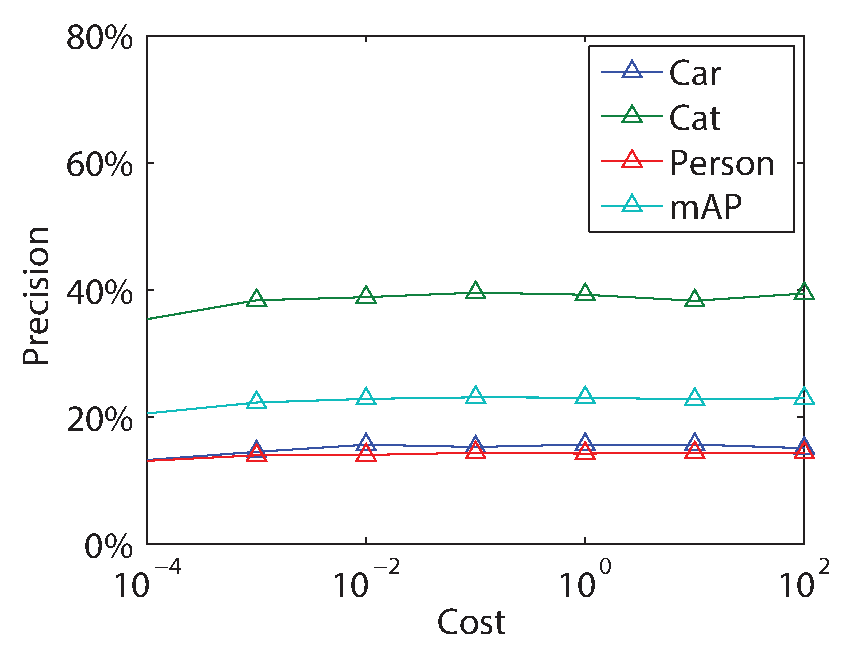
\includegraphics[width=\textwidth]{figures/tuning/cost.eps}
                \caption{SVM Cost}
                \label{fig:cost}
        \end{subfigure}
        ~ 
        \begin{subfigure}[b]{0.24\textwidth}
                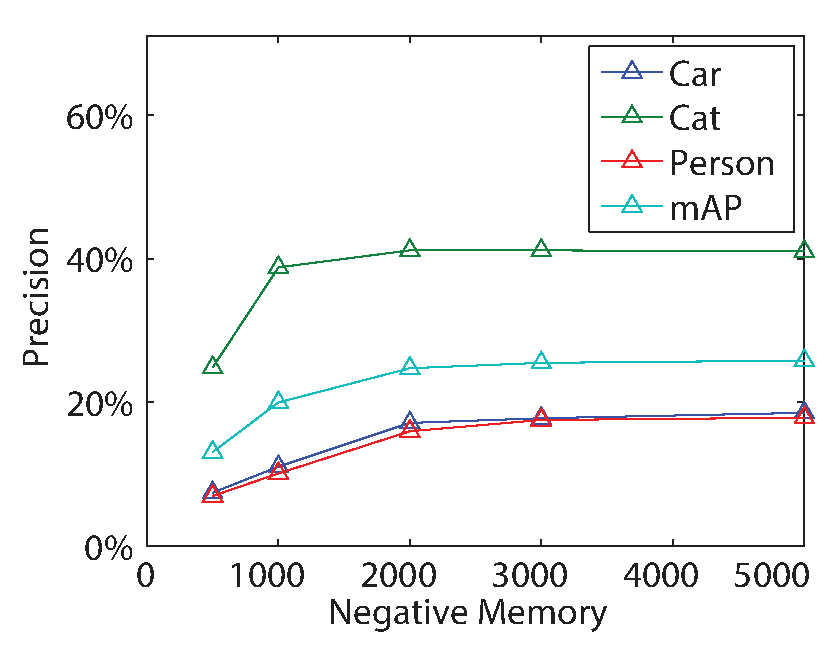
\includegraphics[width=\textwidth]{figures/tuning/negative_memory.eps}
                \caption{Negative Memory}
                \label{fig:negative_weight}
        \end{subfigure}
        ~
        \begin{subfigure}[b]{0.24\textwidth}
        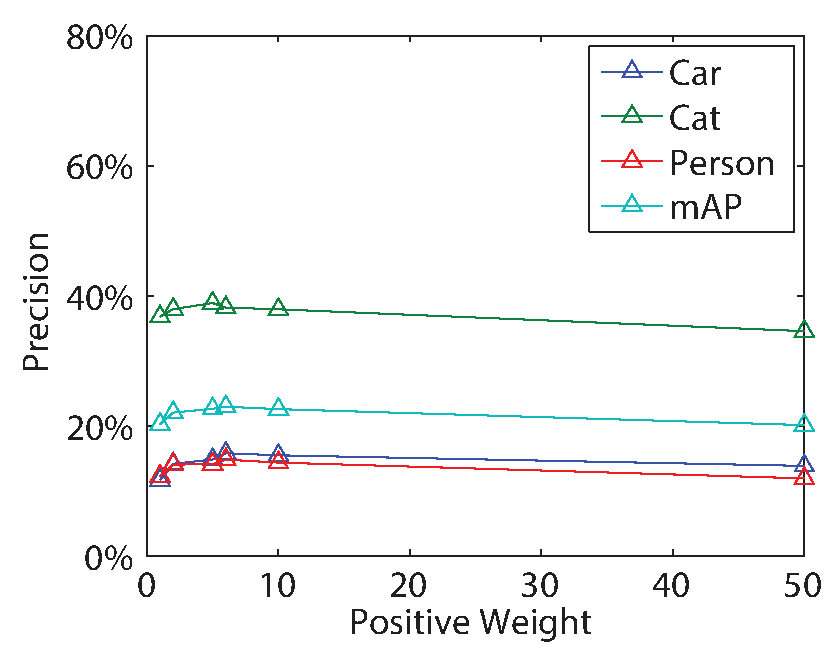
\includegraphics[width=\textwidth]{figures/tuning/positive_weight.eps}
        \caption{SVM Positive Weight}
        \label{fig:positive_weight}
        \end{subfigure}
        
        \vspace{3mm}
        
        \begin{subfigure}[b]{0.24\textwidth}
        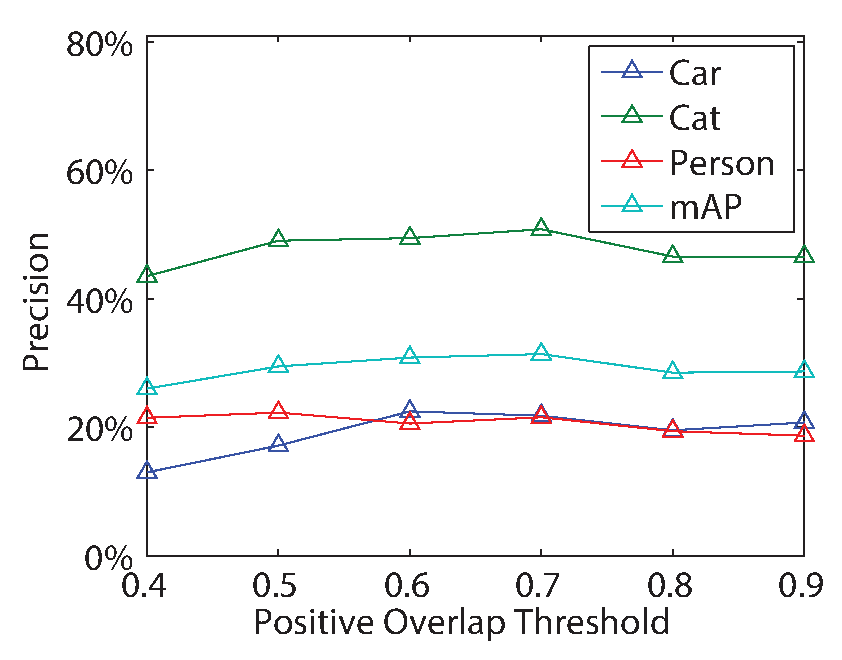
\includegraphics[width=\textwidth]{figures/tuning/pos_overlap.eps}
        \caption{SVM Positive Overlap}
        \label{fig:pos_overlap}
        \end{subfigure}%
        ~ 
        \begin{subfigure}[b]{0.24\textwidth}
                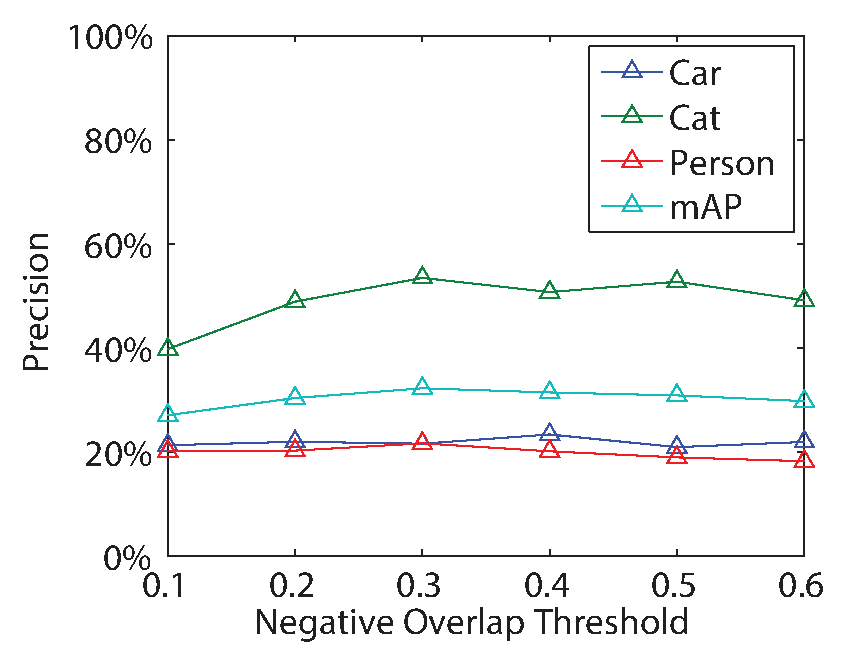
\includegraphics[width=\textwidth]{figures/tuning/neg_overlap.eps}
                \caption{SVM Negative Overlap}
                \label{fig:neg_overlap}
        \end{subfigure}
        ~ 
        \begin{subfigure}[b]{0.24\textwidth}
                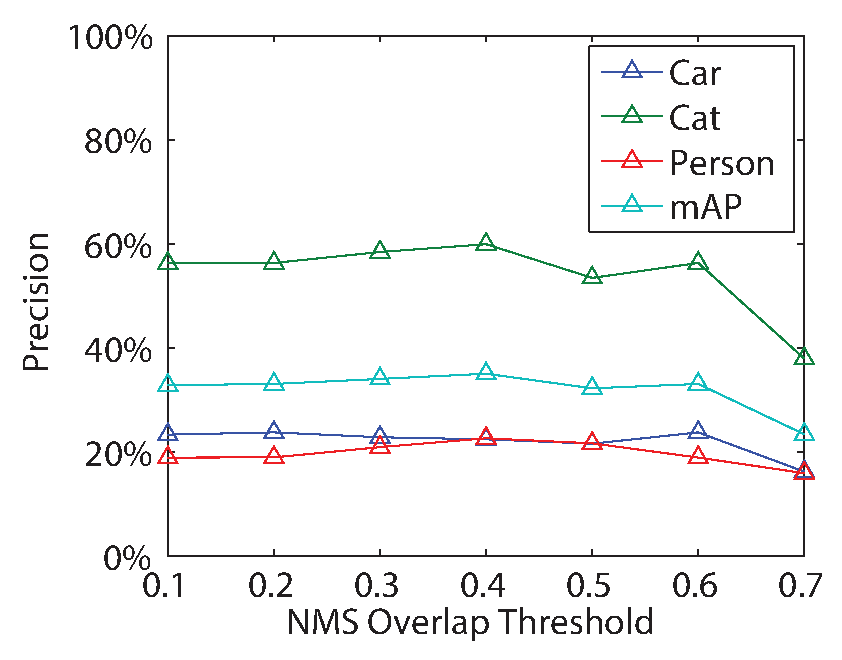
\includegraphics[width=\textwidth]{figures/tuning/nms.eps}
                \caption{NMS Threshold}
                \label{fig:nms_threshold}
        \end{subfigure}
        ~
        \begin{subfigure}[b]{0.24\textwidth}
        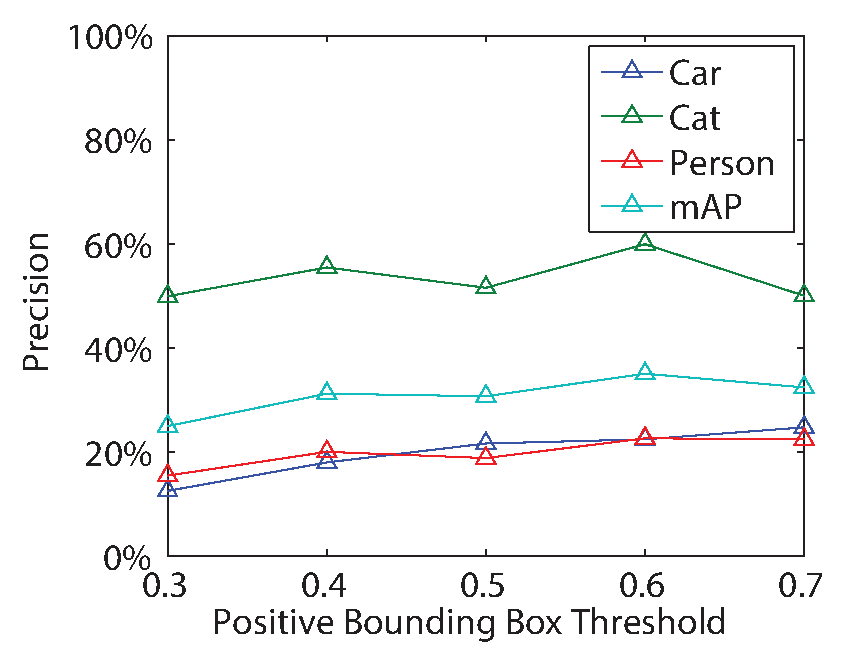
\includegraphics[width=\textwidth]{figures/tuning/pos_bbox.eps}
        \caption{Positive Bbox Overlap}
        \label{fig:pos_bbox}
        \end{subfigure}
        
        \caption{Hyperparameter Tuning Results}\label{fig:hyperparam_tuning}
\end{figure*}

\section{Code Overview}
The code is divided into several files, but all the functionality can be accessed using \texttt{main.py}. All of the code can be found in the \texttt{python} directory. All parameters such as the directories to use for features and models, the CNN properties etc can be set in \texttt{settings.py}. The best hyperparameter values are already set as default in the code. Hence, to get the reported scores, it is sufficient to change the paths in \texttt{settings.py} and to run:
\begin{verbatim}
    python main.py --mode extract
    python main.py --mode train
    python main.py --mode trainbbox
    python main.py --mode test
\end{verbatim}
Extraction mode takes optional arguments such as the number of GPUs to use. To enable bounding box regression, use the \texttt{ --bbox\_regression normal} option when using the \texttt{test} mode. Detailed help is available for each mode upon running \texttt{main.py} with the \texttt{-h} flag. Note that the code depends on the following libraries: \texttt{numpy, opencv, argparse, sklearn, cPickle} and \texttt{pycaffe}. 

For the various source files, \texttt{train\_rcnn.py} contains all the code for using the extracted features and training our classifier. We have code to train both an SVM and an SGD classifier. The file also contains code to evaluate our models on a validation set. The \texttt{test\_rcnn.py} file contains the testing pipeline. It loads the features for the test images, uses the trained classifier and the bounding box regressor, and finally applies non-maximal suppression to output a final set of bounding boxes. The \texttt{det\_eval.py} file is a direct port of the \texttt{det\_eval.m} file provided in the starter code. \texttt{util.py} contains common functions used by all other modules, \texttt{hyperparam\_tuning.m} runs the entire pipeline on various sets of hyperparameters, and finally \texttt{tester.py} tests our ported Matlab functions against their original Matlab implementations (the cross-checking requires that the Matlab Python engine be installed).

\section{Experiments}\label{sec:experiments}

We use the Caffe \cite{jia2014caffe} and cuDNN \cite{chetlur2014cudnn} libraries for our convolutional network implementation. Experiments were performed on three machines:
\begin{itemize}
\setlength\itemsep{0em}
\item Workstation with 32 GiB of main memory and one NVIDIA GTX Titan X GPU with 12 GiB memory
\item Amazon EC2 g2.8xlarge instance with four NVIDIA GRID K520 GPUs with 4 GiB memory each
\item Amazon EC2 r3.8xlarge instance with an Intel Xeon E5-2670 CPU with 256 GiB of main memory
\end{itemize}
Our SVM \cite{scikit-learn} is implemented in liblinear.

\subsection{Features}

As shown in Table \ref{table:features}, the VGG network does not perform as well as JonNet. This could be attributed to two factors: (i) insufficient hyperparameter tuning and (ii) too few training examples with too large of a feature space.

Due to the large network architecture of the VGG network, we were not able to tune the network at the same breadth as JonNet. We hypothesize that much better results can be achieved with further hyperparameter tuning and leave this as future work.

We use the non-rectified layer as our feature representation.  Typically, the fully-connected layers will output 4096 non-zero real values. Since our feature space is much larger than the number of positive examples, this makes the SVM prone to overfitting. The results in Table \ref{table:features} indicate this is a possible explanation for VGG's poor performance. By using the rectified features, many of the 4096 values will become zero and thus will provide less information to the SVM. 

\begin{table}[h]
\centering
\begin{tabular}{llrrrr}
\hline
Network & Features & Car & Cat & Person & mAP \\ \hline
JonNet & fc6\_ft & 21.3\% & 52.3\% & 21.3\% & 31.7\% \\
JonNet+R & fc6\_ft & 22.4\% & 60.0\% & 22.6\% & 35.0\% \\
VGG-16 & fc6 & 7.7\% & 24.7\% & 10.7\% & 14.4\% \\
VGG-16 & fc7 & 8.1\% & 35.6\% & 12.5\% & 18.7\% \\ \hline
\end{tabular}
\caption{Performance of different CNNs and features. 'R' indicates the use of bounding box regression.}
\label{table:features}
\end{table}

As previously mentioned, detection performance depends on the image classification performance. Therefore we hypothesize that the fc7 layer will outperform the fc6 layer due to it's ``higher level" image understanding. This is confirmed in Table \ref{table:features} as the fc7 layer achieves a mAP of 18.7\% while fc6 achieves 14.4\%.

\subsection{Object Classifiers}
As a baseline, we trained classifiers with all negative and positive examples, with a class weight equal to the inverse frequency of the number of examples in that class. We saw no improvement over our hard-mined object classifiers in terms of performance.

After implementing the iterative hard-mining method of reducing the number of negatives, we performed extensive hyperparameter tuning to improve performance. We trained and evaluated all object classifiers on 1,120 different sets of hyperparameters. We modified the regularization costs, the weight on the positive class during SVM training, the maximum number of hard negatives, and the bias term. The results are shown in Figure \ref{fig:hyperparam_tuning}. 

Once we found the optimal set of hyperparameters, we began tuning our model thresholds (e.g. positive and negative overlap thresholds). We also tuned the threshold for rejecting bounding boxes while performing non-maximal suppression. The results are shown in Figure \ref{fig:hyperparam_tuning}.


\subsection{Runtime Performance \& Optimizations}

On a single Titan X GPU, our JonNet feature extraction took 72 minutes. Before we process each selective search proposal, we need to preprocess it to meet the requirements of the CNN. This process is CPU intensive, and hence parallelizing this portion of the extraction process gave us a significant boost in performance. VGG feature extraction, in parallel, took a total of 3 hours.

\subsection{Error Analysis}
Looking at the qualitative results, we do very well on the cat class. Our model has a difficult time with the other two classes. One reason for this might be because our original CNN was trained on images with a lot of cats in them. We can still see some very nice results in Figure \ref{fig:successful_images}, for example, in the third successful image, the classifier is able to identify the cars using very small portions - the tail lights for one of the cars, and the side door for the other one. This was expected, as a lot of our training images are cars captured from the back and the side.
On the unsuccessful cases, we notice that we have a lot of false positives for the person class. This is expected with the relatively small dataset size we had, as there are a lot of variations in people (different clothing styles and colors, various poses etc). We also sometimes detect false positives for cats, especially where there is a uniformly colored texture - like clothing. An example of this can be seen in the fourth difficult image example in Figure \ref{fig:unsuccessful_images}. This can be attributed to the fact that because of their weird poses, cats sometimes appear as a uniformly textured blob.
\begin{figure*}[t]
	\vspace{-5mm}
	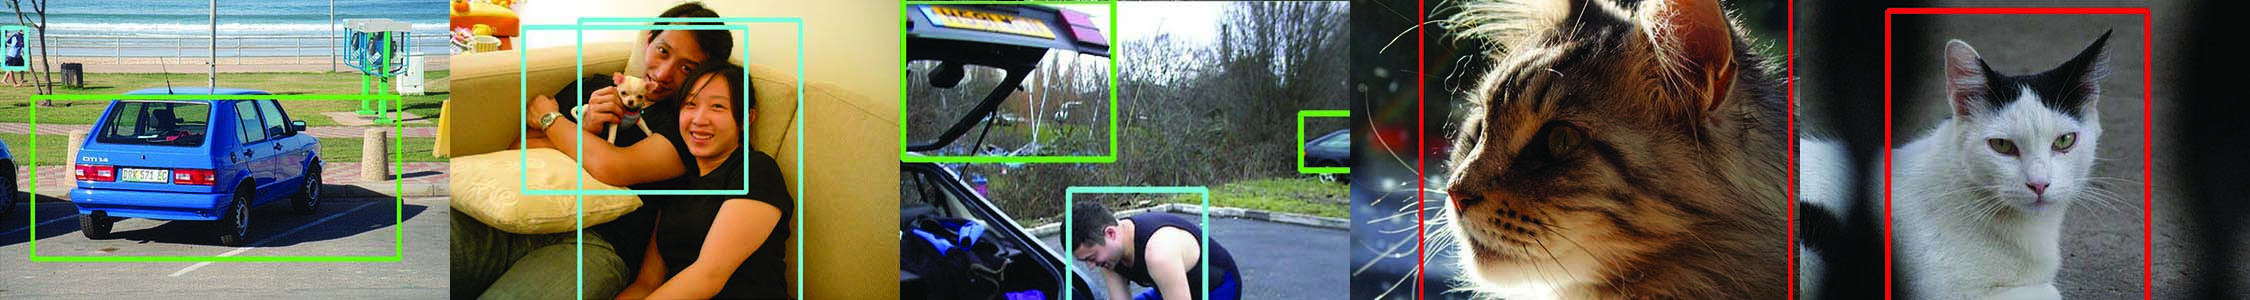
\includegraphics[width=\textwidth]{figures/qualitative/all_good.jpg}
	\caption{Successful images. Red, green, and cyan bounding boxes correspond to the cat, car, and person classes, respectively.}
	\label{fig:successful_images}
	\vspace{4mm}
	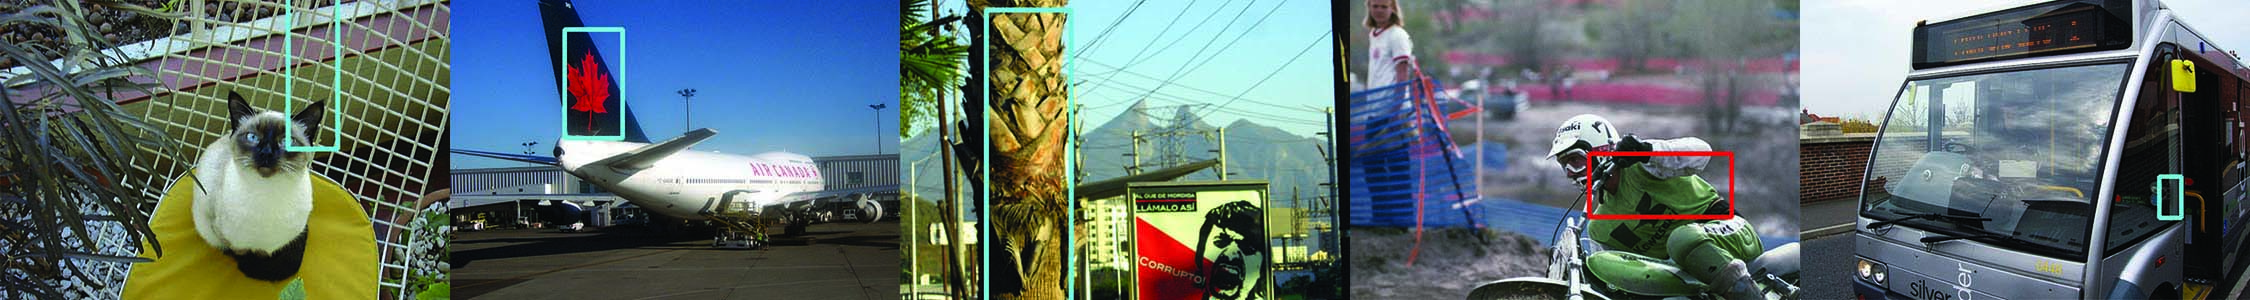
\includegraphics[width=\textwidth]{figures/qualitative/all_bad.jpg}
	\caption{Difficult images. Red, green, and cyan bounding boxes correspond to the cat, car, and person classes, respectively.}
	\label{fig:unsuccessful_images}
\end{figure*}

\section{Extensions}

\subsection{Bounding Box Regression}

\begin{figure*}[t]
	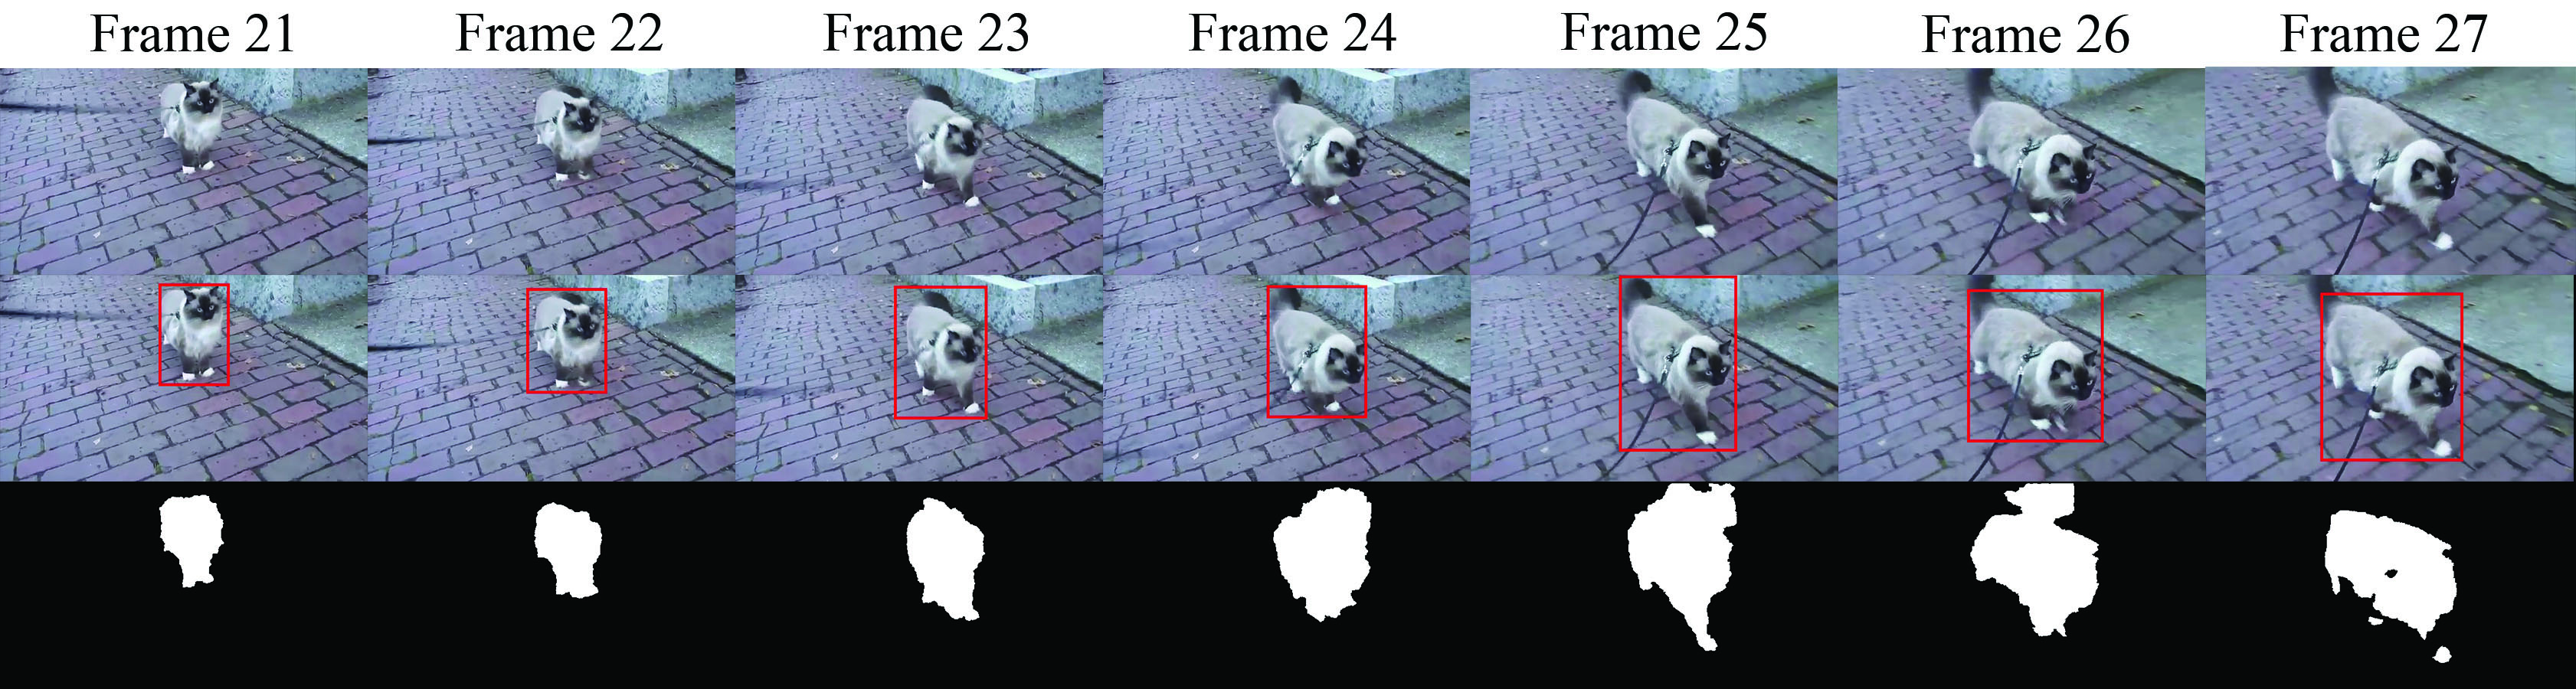
\includegraphics[width=\textwidth]{figures/cat_video.jpg}
	\caption{Foreground object detection with GrabCut image segmentation.}
	\label{fig:grabcut}
\end{figure*}

	\textbf{Multivariate Ridge Regression}.	To improve localization performance, Girshick \etal propose four SVMs using the ridge regression formulation:
	\begin{equation}\label{eq:single_regression}
	\mathbf{w}_\star = \underset{w_\star}{\textrm{argmin}} \sum_{i}^{N} (t_\star^{(i)} - \mathbf{w}_\star^T \phi(P^{(i)}))^2 + \alpha || \mathbf{w}_\star ||^2
	\end{equation}
	where $\mathbf{w}_\star$ denotes the vector of learned model parameters and $\star$ is one of $x,y,h,w$, and $\phi(P^{(i)})$ denotes the extracted features for proposal $P^{(i)}$, and $N$ is the number of proposals.
	We generalize Equation \ref{eq:single_regression} to the multiple-target (\ie multi-variate) case:
	\begin{equation}\label{eq:multivariate_regression}
	\mathbf{w} = \underset{w}{\textrm{argmin}} \sum_{i}^{N} || \mathbf{t}^{(i)} - \mathbf{w}^T \phi(P^{(i)})||^2 + \alpha || \mathbf{w} ||^2
	\end{equation}
	where  $\mathbf{t}$ is now a vector composed of four targets. Notice that we now have a single $\mathbf{w}$ per class, as opposed to four. The results are shown in Figure \ref{fig:alpha}.

    \textbf{Support Vector \& Elastic Net Regression}. In addition to the ridge regression, we experiment with the support vector regression and elastic net regression. The support vector regression is similar to a SVM classifier but instead outputs real values. To further experiment with the regularization parameter, we use an Elastic Net regression \cite{zou2005regularization} to combine both a $\ell_1$ and $\ell_2$ regularizer. The objective function is defined in Figure \ref{fig:elastic_net}.
\begin{figure*}[t!]
\vspace{-4mm}
\begin{equation*}
w = \underset{w}{\textrm{argmin}} \frac{1}{2N} \sum_{i}^{N} || \mathbf{t}^{(i)} - \mathbf{w}^T \phi(P^{(i)})||^2_2 + \alpha \rho || w || + \frac{\alpha (1-\rho)}{2} || w ||^2_2
\end{equation*}
\caption{Optimization problem for the Elastic Net regression. It uses both $\ell_1$ and $\ell_2$ regularizers.}
\label{fig:elastic_net}
\end{figure*}
where $0 \leq \rho \leq 1$ controls the strength of the $\ell_1$ and $\ell_2$ regularization term. We set $\rho=0.5$.

\textbf{Alpha Sensitivity}. Additionally we evaluate the sensitivity of mAP to $\alpha $. The results are shown in Figure \ref{fig:alpha}. For large values of $\alpha$, mAP increases until 10e4 then begins to decrease. We can attribute this decrease to the fact that large values of $\alpha$ reduce the variance of our predictions in ridge regressions. It might be possible that because of reduced variance, our regressor does not provided optimal offsets to the correct bounding box, thus reducing our overall accuracy.


\begin{figure}
        \centering
        \begin{subfigure}[b]{0.24\textwidth}
                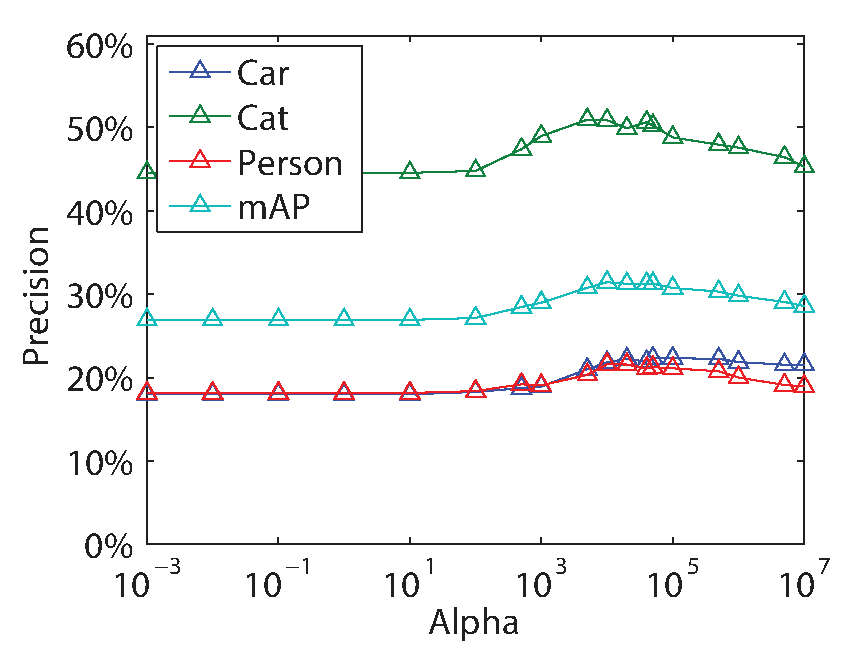
\includegraphics[width=\textwidth]{figures/tuning/alpha.eps}
                \vspace{0.2mm}
                \caption{Alpha}
                \label{fig:alpha}
        \end{subfigure}%
        ~ 
        \begin{subfigure}[b]{0.24\textwidth}
                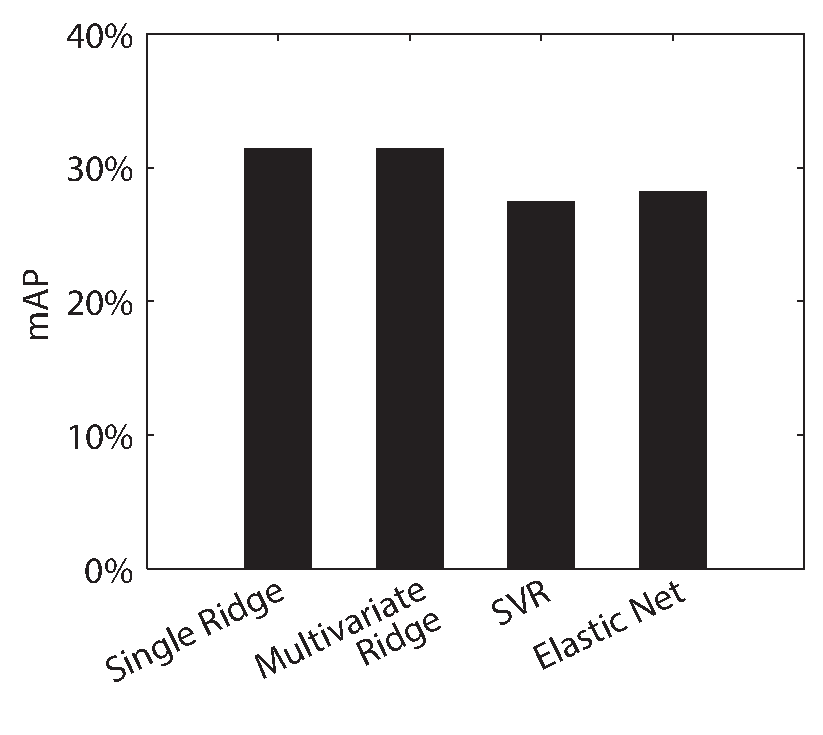
\includegraphics[width=\textwidth]{figures/tuning/regressions.eps}
                \caption{Linear Regressions}
                \label{fig:linear_regressions}
        \end{subfigure}
        \caption{Results of bounding box regression tuning}
\end{figure}


    
\subsection{Individual Parameter Tuning}
While using the same hyperparameters for all of the object classifiers reduces the overall effort, we wanted to see if there is a significant difference if we tuned each of the classifiers individually on their own set of hyperparameters. These tests were run before we tuned our bounding box regression and thresholds. Although there is an improvement for the cat class, surprisingly there is no significant improvement for the other classes as seen in table \ref{table:individual_params}. One reason for this might be better features for the cat class, since the CNN was trained on ImageNet, which has a lot more cats than cars and people. 
\begin{table}[h]
\centering
\begin{tabular}{lcc}
\hline
 & Shared Parameters & Individual Parameters  \\ \hline
Car & 22.3\% & 22.5\% \\
Cat & 43.4\% & 48.1\% \\
Person & 21.8\% & 21.8\% \\ \hline
\end{tabular}
\caption{Precision (shared vs individually-tuned)}
\label{table:individual_params}
\end{table}

\subsection{SGD Classifier}
We implemented and tuned an SGD Classifier instead of the standard SVM. The advantage to this was that we could train on the entire dataset with limited memory. We collected positives and negatives from small batches of images, and trained the classifier incrementally. After tuning the class weights and regularization penalties, we achieved a 80\% accuracy on our validation set, but do poorly on the object detection task (15 AP for cat class). We also needed to tune the parameters for each class individually in this case, which might suggest that classifier was overfitting on our training data. This would also explain the poor performance on the overall object detection.

\subsection{Foreground Extraction from Video}

As an additional extension, we use the output bounding box of our R-CNN as input into GrabCut. Since our algorithm successfully detects cats, we apply our algorithm to a video of a cat walking outdoors.\footnote{\url{https://www.youtube.com/watch?v=oYTUfM1vEjs}} We pass each frame of our video through the CNN for feature extraction. Using the original selective search code, we extract between 300 to 1000 region proposals per frame. Due to the high performing cat classifier and regression, our R-CNN returns a single bounding box for all frames. This bounding box is passed as input into GrabCut which is then run for 10 iterations. No user interaction is required at any point in the detection or segmentation process.


The results are viewable online.\footnote{\url{http://albert.cm/cs231b/p3/}} The video contains the original frames, R-CNN bounding boxes, and foreground silhouettes. A subset of the results are shown in Figure \ref{fig:grabcut}.

%\begin{itemize}
%\item Multivariate bbox regression
%\item $\ell_2$ normalization for features instead of ZMUV
%\item Foreground extraction from video (of cat or cars) using GrabCut algorithm
%\item A theoretical extension maybe. Albert will ponder this on the plane
%\item Individually tuned SVMs vs Shared parameters
%\end{itemize}

%\newpage
%\balance
{\small
\bibliographystyle{ieee}
\bibliography{egbib}
}

\end{document}
